

\chapter{Le son et sa définition}
\section {Unités de mesures}
Un décibel\autocite[In Wikipedia]{noauthor_decibel_2018} (\SI{}{\decibel} ) est l'unité de mesure de l'intensité du son.
 Un décibel est égal à $1/10$ de bel (\SI{}{\bel}):
	$$\SI{1}{\decibel} = \SI{1/10}{\bel} $$
	 Une augmentation de l'intensité égale à \SI{1}{\bel}
équivaut à peu près à un doublement de l'intensité sonore.
		
Un hertz (\si{\hertz}) est une unité de fréquence\footnote{La fréquence est le nombre de vibrations par unité de temps dans un
		phénomène périodique.}. Équivalent à $\SI{1}{\second - 1} $. Fréquence d'un phénomène périodique
	dont la période est une seconde. \pdfmargincomment{Je laisserais tomber les multiples etc.} Ses multiples sont, entre autres,
	le kilohertz (\si{\kilo\hertz}), le mégahertz (\si{\mega\hertz}) et le gigahertz (\si{\giga\hertz}). Cette
	unité vient du savant allemand Heinrich Hertz, pionnier de la radioélectricité.

\subsection{Deux façons de définir le son et l'écoute}



De manière objective:
C'est le phénomène phy\-si\-que
d'origine mécanique consistant en une variation de pression (très
faible), de vitesse vibratoire ou de densité du fluide, qui se propage
en modifiant progressivement l'état de chaque élément du milieu considéré,
donnant ainsi naissance à une onde acoustique.

De manière subjective:
	Il s'agit de la sensation procurée
	par cette onde, qui est reçue par l'oreille, puis transmise au cerveau
	et déchiffrée par celui-ci.\footnote{www.futura-sciences.com \pdfmargincomment{Page stp?}} 
	\index{http://www.futura-sciences.com/sante/dossiers/medecine-bruit-effets-sante-259/page/3}

Il faut aussi tenir compte de  l'impression de force sonore : la sensibilité de l'oreille
est une variable de la fréquence. Il faut 1000 fois moins de pression
acoustique pour avoir une sensation auditive à \SI{4000}{\hertz} qu'à \SI{50}{\hertz}.
Notre oreille n'a donc pas la même sensibilité pour toutes
les fréquences audibles. Il en est de même pour la sensation auditive
des basses fréquences et pour la dynamique. 


\chapter {Anatomie de l'oreille}

\section {L'oreille}


\begin{quotation}
	\char`\"{}\textbf{C'est le son qui a fabriqué l'oreille et si tu veux connaître
		le son, apprends d'abord à étudier l\textquoteright
                oreille\char`\"{}.}

              
	Hermès Trimégiste 
\end{quotation}

\subsection{L'anatomie de l'oreille}
\begin{figure}
	\centering
	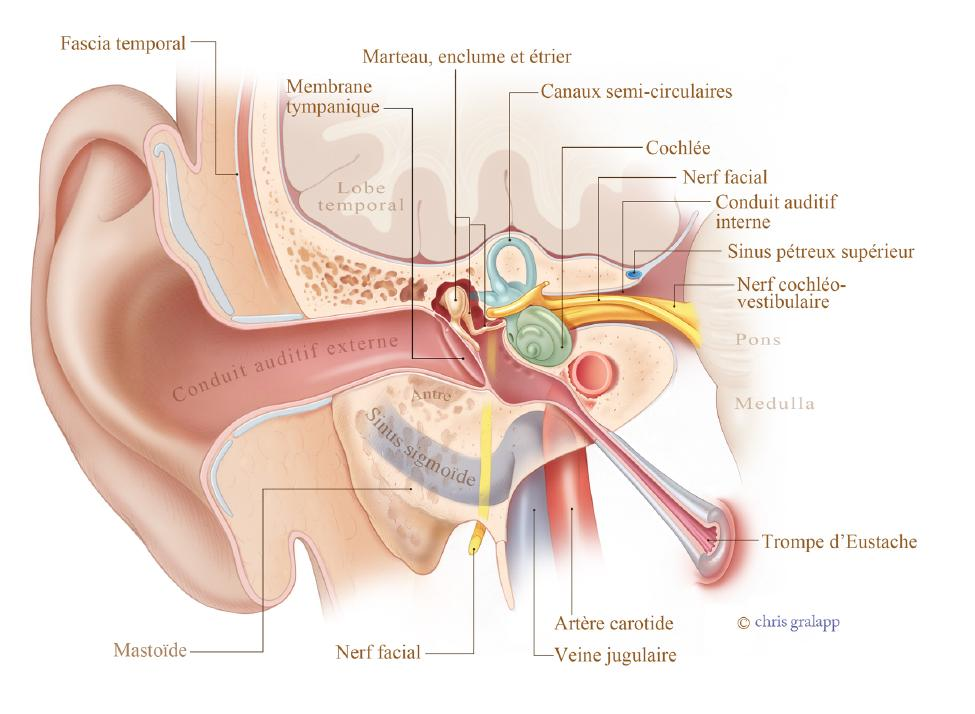
\includegraphics[width=1\linewidth]{images/20160624Berufsfeldgruppen.jpg}
	\caption[Anatomie oreille]{Anatomie de l'oreille}
	\label{fig:-20160624berufsfeldgruppen}
\end{figure}

L'oreille \autocite[ch. 8 pp. 319--321]{marieb:biologie} 
se situe à l'intérieur de l'un des os du crâne, le temporal, et plus précisément la pyramide pétreuse ou rocher. Elle se compose de trois parties : externe, moyenne, interne.

\subsubsection{L'oreille externe}

L'oreille externe\autocite[ch. 8, pp. 319--321.]{marieb:biologie}
est formée du pavillon et du méat acoustique externe
	(canal auditif). Les ondes sonores entrent dans le méat et percutent
	une membrane de \SI{60}{\milli\metre\squared}, appelée tympan, et la font vibrer. 
	Cette membrane
	sépare l'oreille externe de l'oreille moyenne. 


        Selon \textbf{Tomatis} 
	% au chapitre 3.3/ 4, 
	elle joue un rôle de filtre des graves et d'amplificateur des aigus.




\subsubsection{L'oreille moyenne}

L'oreille moyenne se trouve dans l'os temporal constituée de petites
cavités dont une, centrale, qui est la caisse du tympan. Sa limite
médiale est une paroi osseuse percée de deux orifices, la fenêtre
du vestibule et la fenêtre de la cochlée. La trompe auditive ou d'Eustache
est un conduit oblique qui relie l'oreille moyenne à la gorge et sert
à équilibrer la pression de l'air entre l'oreille moyenne et l'extérieur.
Les trois osselets de l'ouïe sont : le marteau, l'enclume et l'étrier
(les plus petits os du corps). Ils transmettent les vibrations du
tympan aux liquides de l'oreille interne.
Le marteau et l'étrier sont commandés chacun par un muscle.


Selon \textbf{Tomatis}, son rôle est double : protéger l'oreille interne des sons
trop forts et celui de cibler les sons à écouter.

\subsubsection{L'oreille interne et le labyrinthe osseux}

\begin{figure}
	\centering
	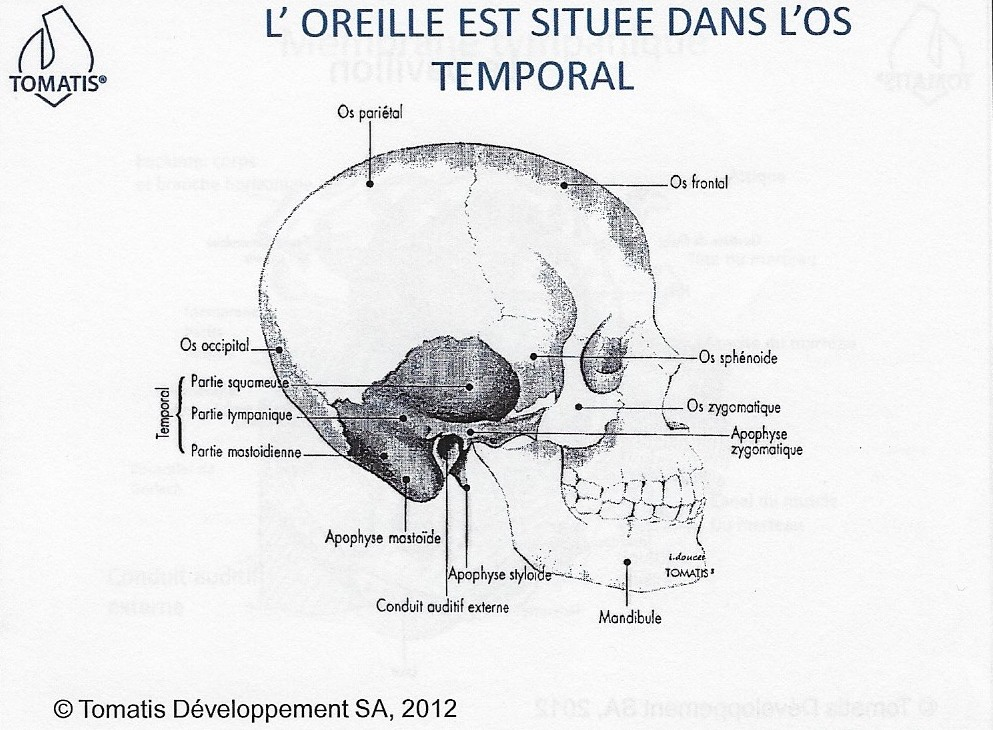
\includegraphics[width=0.7\linewidth]{images/Loreilleostemporal_crane.jpg}
	\caption[L'os temporal]{L'os temporal}
	\label{fig:loreilleostemporal18}
\end{figure}

L'oreille interne est l'organe de l'audition. Il
est constitué d'une coque osseuse d'une très grande densité (la plus
importante du corps), contenant un corps membraneux qui en épouse
la forme. 
L'oreille interne est une enfilade de cavités osseuses portant 
le nom de \emph{labyrinthe osseux}. Il comprend trois subdivisions : 
\begin{enumerate}
	\item la cochlée;
	\item le vestibule du labyrinthe;
	\item  les canaux semi-circulaires.
\end{enumerate}

Le labyrinthe
osseux est rempli de périlymphe, un liquide. Et dans ce périlymphe
flotte le labyrinthe membraneux qui contient lui-même un liquide
plus épais appelé endolymphe. Ils jouent leur rôle dans l'équilibre
statique et dynamique. Le vestibule et les canaux semi-circulaires
sont les organes de l'équilibration; la cochlée ou
limaçon est l'organe de l'audition. 

\subsubsection{Le canal auditif}
\pdfmargincomment[color=yellow]{répétition avec oreille externe}
Les ondes sonores entrent dans le méat et percutent
une membrane de \SI{60}{\milli\metre\squared} appelée \emph{tympan}, et la font vibrer. Cette membrane
sépare l'oreille externe de l'oreille moyenne.


Selon \textbf{Tomatis}, elle
joue un rôle de filtre des graves et d'amplificateur des aigus.



\subsection{La physiologie de l'audition}

Le  son crée un chemin dans 
l'oreille\autocite[chap. 8, pp. 322--324]{marieb:biologie} jusqu'au cerveau.

Chaque son parvenant à l'oreille entre dans le pavillon et se propage
dans le conduit auditif. Les vibrations de l'onde sonore mettent en
mouvement le tympan lié aux trois petits os (marteau, enclume, étrier).
Les osselets ont le rôle de transformer et d'amplifier les vibrations
aériennes et de les transmettre à l'oreille interne via la fenêtre
ovale.

Le rapport de levier effectif entre le marteau et l'enclume
(de l'ordre de 20), d'une part, et le
rapport de surfaces entre le tympan et la platine de l'étrier
(\SI{30}{\milli\metre\squared}) d\textquoteright autre part font du système tympano-ossiculaire
un véritable amplificateur permettant à l\textquoteright énergie sonore
d\textquoteright être transmise presque intégralement à l\textquoteright oreille
interne.

A partir de 80 dB, un réflexe protecteur (stapédien) est mis en place
afin de réduire la transmission des pressions vers l\textquoteright oreille
interne, par l\textquoteright intermédiaire des osselets et des muscles
qui rattachent le marteau et l\textquoteright étrier aux parois de
la caisse du tympan. Il s'agit ainsi d' un procédé mécanique qui amplifient
les vibrations atteignant la cochlée. 
\begin{quotation}
	La cochlée à son tour ``va transformer ces vibrations en impulsions
	nerveuses véhiculées par le nerf auditif.'' (\dots) Les cellules ciliées
	tapies dans la membrane cochléaire ``transforment ces vibrations
	en messages électriques, circulant dans le nerf auditif. (\dots) Et
	ces informations vont ``se diriger vers le cortex cérébral, via plusieurs
	relais. (\dots) ``Comme certaines fibres issues de chaque oreille croisent
	la ligne médiane, chaque aire auditive reçoit des signaux des deux
	oreilles.'' De plus, ``tout au long du trajet, le message subit
	des transformations dues aux caractéristiques de l'activité des neurones.''
	Retenons que `` les cellules ciliées proches de l'étrier sont activées
	par les sons aigus, et celles situées au sommet de la cochlée le sont
	par les sons de basse fréquence''. (\dots)``Une scène auditive est
	mêlée d'un ensemble d'ondes acoustiques et son analyse se ferait non
	seulement tout au long du système auditif avec des indices comme la
	fréquence et l'intensité mais aussi au-delà, pour utiliser les informations
	liées aux autres sens ou au contexte.'' \autocite[chap.1, pp.~15--16]{bigand:cerveau}
%	\footnote{\textbf{Le cerveau mélomane} Le cerveau mélomane,2011}, chap.1, pp.~15--16.}
\end{quotation}


        \begin{figure}
	\centering
	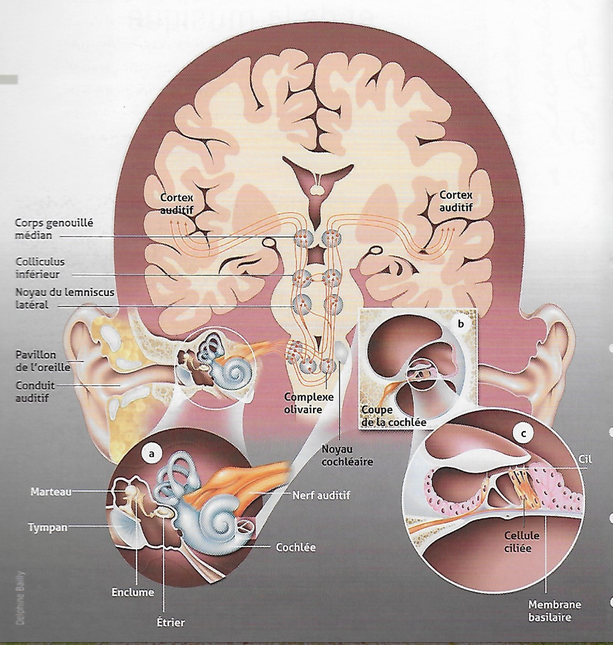
\includegraphics[width=1\linewidth]{images/schemacerveauoreillebigand.png}
	\caption[Schéma du déroulement]{La perception des sons et de
          la musique, E.Bigand, ``Le cerveau mélomane''Ed.Belin}
       
	\label{cerveauoreillebigand1}
\end{figure}




\chapter{Acoustique}

\section{Courbe de Wegel}
\label{acoustique}

<<Effectivement la courbe de Wegel est la courbe de réponse obtenue
lorsque sont posées en abscisses les fréquences, et en ordonnées ascendantes
les intensités. Un premier seuil s'obtient, en partie basse, suivant
un minimum qui commence dans les fréquences graves à environ 
\SIrange{40}{50}{\dB}, avoisine ensuite la courbe des abscisses entre 2000 et \SI{3000}{\Hz}
et redevient ascendante à \SI{40}{\decibel} / \SI{50}{\decibel} dans les aigus entre \SI{8000}{\Hz} et
\SI{10000}{\Hz}. Cette courbe se complète et prend l'allure de citron selon
l'expression qu'on lui confère lorsqu'on envoie des
sons d'intensité croissante et qu'on obtient alors une courbe des
seuils maxima qui se déterminent là où l'oreille commence à souffrir,
d'où le nom de ``seuil de la douleur". Ces seuils
commencent dans les graves, également de \SIrange{50}{60}{\decibel}, rejoignant la première
courbe, puis ils atteignent \SIrange{120}{130}{\decibel} entre \SI{2000}{\Hz} et \SI{3000}{\Hz} pour
chuter ensuite dans les aigus en rejoignant également la première
courbe. La ligne médiane qui se situe aux environs de \SIrange{50}{60}{\dB}, qui
est linéaire représente une zone dite ``Zone de Munsen''.
Elle répond à la dynamique de l'oreille, c'est-à-dire
à sa zone ``optimale" de fonctionnement sans
distorsion. Dans toutes les autres zones, l'oreille
agit comme un filtre dont les pentes sont variables en fonction de
l'intensité, avec un lieu de rotation situé de \SIrange{1000}{2000}{\Hz}. Pour pallier ces distorsions toujours difficiles à intégrer
dans la lecture des schémas, les Américains ont standardisé les audiogrammes
du type de ceux que nous utilisons tous en inversant l'image
de Wegel et en redressant les \emph{minima} pour obtenir une ligne droite.
Ces normes gardent néanmoins une zone préférentielle de \SIrange{1000}{2000}{\Hz} malgré les compensations de \SIrange{30}{40}{\dB} accordées sur la courbe,
dans les graves et les aigus.>>
\autocite[Bernard Auriol, conversation, conférence]{auriol_stress}.

% OGA: stp la source bibliographique ou conférence

\section{Impédance}
\label{impedance}

Définition de l'impédance : L'impédance acoustique
caractérise la résistance qu'un milieu oppose à sa mise en mouvement
lorsqu'il est traversé par une onde acoustique. Elle est définie comme
le rapport de la pression acoustique sur la vitesse de déplacement
locale dans un milieu, et est généralement notée $Z$. Elle dépend de
la température. L'impédance caractéristique d'un milieu (solide, liquide
ou gazeux) est définie comme le rapport de la pression acoustique
sur la vitesse de déplacement en milieu ouvert (c'est-à-dire
en l'absence d'ondes réfléchies). L'impédance caractéristique est
une propriété du matériau considéré égale, dans le cas d'un espace
illimité, au produit de la masse volumique du matériau $\rho$
par la vitesse du son $c$ dans ce même matériau : $Z = \rho_{m} c$.

Unités : $\rho_{m}$ étant exprimé en \si{kg/m\cubed},
$c$ en \si{m/s}, $Z$ est
exprimé en \si{\pascal . s/m}.



\textbf{Technique de travail sous ``Oreille électronique''}
Le but de cet appareil 
est de modifier la manière d'entendre. On oblige l'oreille à utiliser
un mode d'accommodation qui 
détermine une manière d'entendre typique et entraîne le geste
vocal correspondant.
L'oreille va donc se tendre
vers l'information qui lui arrive, entraînée par l'Oreille
électronique qui lui fait faire une
gymnastique très précise.

 L'adaptation de l'oreille moyenne se fait par le jeu des contractions
du muscle du marteau et du muscle de l'étrier.
\begin{itemize}
\item Le muscle du marteau agit sur la convexité imposée au tympan, qui
se comporte alors comme une lentille acoustique, sorte de cristallin
auditif. \item Le muscle de l'étrier régule le jeu de l'oreille interne, qui sait,
à la manière d'un prisme, étaler la gamme des sons en spectre acoustique.
\end{itemize}}

L'Oreille Electronique impose ce jeu à l'oreille avec le jeu de
bascule \footnote{Cf. explication au point \ref{bascule}, p. \pageref{bascule}.}  sur des musiques préparées.

Pour stimuler le désir d'écoute
du patient, il est aussi possible de préparer des musiques avec une
technique particulière, dénommée \emph{retard}, agissant sur le muscle de
l'étrier, c'est-à-dire sur la conduction osseuse. Une autre technique
est celle de la \emph{précession}, qui aidera à viser et décoder les messages,
en agissant sur le tympan, c'est-à-dire sur la conduction aérienne.
Il s'agit donc, comme nous pouvons le constater, d'un assemblage très
fin de techniques. 

\chapter{Feuille informative de l'étude faite à la Privatklinik von Meiringen}
Voici la version originale en allemand proposée aux patients:
\begin{german}

Information für Mitwirkende an der klinischen Studie
\foreignquote{german}{Evaluierung des aktiven Hörvermögens}


Sehr geehrte Damen und Herren,

Herzlichen Dank für Ihr Interesse an dieser Studie !

Wozu dient diese Studie und weshalb werden Sie um eine Teilnahme gebeten ?

Während Ihrem Klinikaufenthalt  in der Privatklinik von Meiringen werden Sie im Kontext 
unseres multidisziplinären Teams verschiedene Therapien besuchen, unter anderem auch die Musiktherapie. Bei der vorliegenden Studie möchten wir untersuchen, wie sich die Musiktherapie auf Ihr Zuhörvermögen auswirkt.
Musiktherapie ist eine gut erforschte Intervention im Bereich des Depressions und Burnouts, da Sie ein relativ neues Berufsfeld ist, gibt es noch viel Forschungspotential.
Das Hörtest konnte sich als ein Instrument erweisen, um die Veränderung des Gehörs des Patienten bei einer Musiktherapiebehandlung zu beweisen. Die Verbindung dieses Ansatzes mit der Musiktherapie ist noch nicht erforscht und daher soll dieser Ansatz wissenschaftlich näher untersucht werden.
Wenn Sie keine Musiktherapie besuchen aber Interesse für diese Studie haben, sind Sie herzlich eingeladen, dieses Test zu tun. Im Rahmen under MAS brauchen wir unbedingt eine Kontrollgruppe.

Wie sieht eine Teilnahme an der Studie aus ?

Die Untersuchung erfolgt sehr einfach in mehreren Schritten.
Zu Verfügung steht ein Apparat, mit dem sich spezifische Hörtests durchführen lassen.
Allgemein Verlauf des Tests :  
Sie hören einen sehr leisen Ton mit Zuhörern zu und werden ihn entweder mit der rechten  oder linken Hand  signalisieren. Das dauert ungefähr 30 Minuten.
Es wird zwei Tests geben : ein vor der Therapie und ein nach der Therapie.
Wir bitten Sie auch, eine kleine Fragebogen zu erfüllen.


Falls Sie Fragen haben, dürfen Sie sich gerne via E-Mail melden : valerie.gaillard\@gmx.ch

Wir bedanken uns herzlich für Ihre Zeit und die Teilnahme an dieser Studie.

\end{german}
Valérie Gaillard


\textgerman{ZhdK : Upgrade MAS Klinische Musiktherapie 15-17}

\section{Feuille informative en français de l'étude faite à la Privatklinik von Meiringen}

Information pour les participants à l'étude clinique
\foreignquote{french}{Evaluation de la capacité de l'écoute active}


Mesdames et Messieurs,

Tout d'abord un très grand merci pour votre intérêt à cette étude!

Dans quels buts et pour quelles raisons êtes-vous priés de participer à
cette étude?

Pendant votre séjour à la clinique de Meiringen, vous allez prendre
part dans le contexte multidisciplinaire à différentes thérapies, dont
la musicothérapie. Avec l'étude présente, nous aimerions étudier comment
la musicothérapie agit sur vos capacités d'écoute.
La musicothérapie fait partie des interventions indiquées et explorées dans le domaine
de la dépression et du burnout; comme c'est un champ
professionnel
relativement nouveau, (il existe un grand potentiel de recherche.) nous avons encore de grandes possibilités d'investigation.
Le test d'écoute pourrait être un instrument prouvant et démontrant le changement
d'écoute du patient lors d'un traitement en musicothérapie.
Le lien de cette approche avec la musicothérapie n'a pas été encore
investigué et c'est la raison pour laquelle elle mérite d'être
recherchée beaucoup plus en profondeur.

Si vous ne suivez aucune musicothérapie mais que vous êtes intéressés
par cette étude, vous êtes invités cordialement à faire ce test. Dans
le cadre de ce travail, il est nécessaire d'avoir un groupe de contrôle.

Comment se présente une participation à cette étude ?

L'étude se déroule très simplement en plusieurs étapes:
À disposition se tient un appareil, avec lequel se fait un test spécifique d'écoute.

Déroulement général du test :
Vous entendrez  avec des écouteurs un son de très faible intensité, que
vous devrez signaler avec la main droite ou gauche, du côté
perçu.
Le tout dure environ 30mn.
Il y aura 2 tests: un avant la thérapie et l'autre après, et à chaque
fois, il sera nécessaire de remplir un petit questionnaire.
Nous vous prions également de signer votre consentement avant le début
de l'étude.


Au cas où vous avez des questions, écrivez-les par E-Mail à cette adresse : valerie.gaillard\@gmx.ch

Nous vous remercions d'ores et déjà beaucoup pour votre participation
à cette étude.

Valérie Gaillard


\begin{french}
	Le matériel utilisé : une table, deux chaises, l'appareil
	test Hearing et les deux écouteurs: l'un aérien et l'autre osseux, un crayon, deux
	feutres (rouge et bleu), une feuille avec la grille de fréquences à
	remplir.
\end{french}

\chapter{WHOQO--Bref: World Health
   Organisation Quality of Life Assessement}

Le WHOQO--Bref (World Health
   Organisation Quality of Life Assessement) est ici reproduite en
   français et en
   version allemande, telle qu'elle a été présentée aux patients.

\includepdfmerge{French_WHOQOL-BREF.pdf, -, 
 WHOQOLALLEMANDBREFupdated.pdf, -}

Le WHOQO--Bref (World Health
   Organisation Quality of Life Assessement) est ici reproduite en
   français et en
   version allemande, telle qu'elle a été présentée aux patients.

\chapter{Déclaration de consentement}

\begin{figure}
	\centering
	\includegraphics[width=1\linewidth]{images/einverstandniserkl.jpg}
	\caption{Déclaration de consentement écrite concernant la
          participation à l'investigation}
	\label{fig:déclaration de consentement}
\end{figure}
%\includepdfmerge{French_WHOQOL-BREF.pdf, -}
%\includepdfmerge{WHOQOLALLEMANDBREFupdated.pdf, -}

%\section{Questionnaire 1}
%
%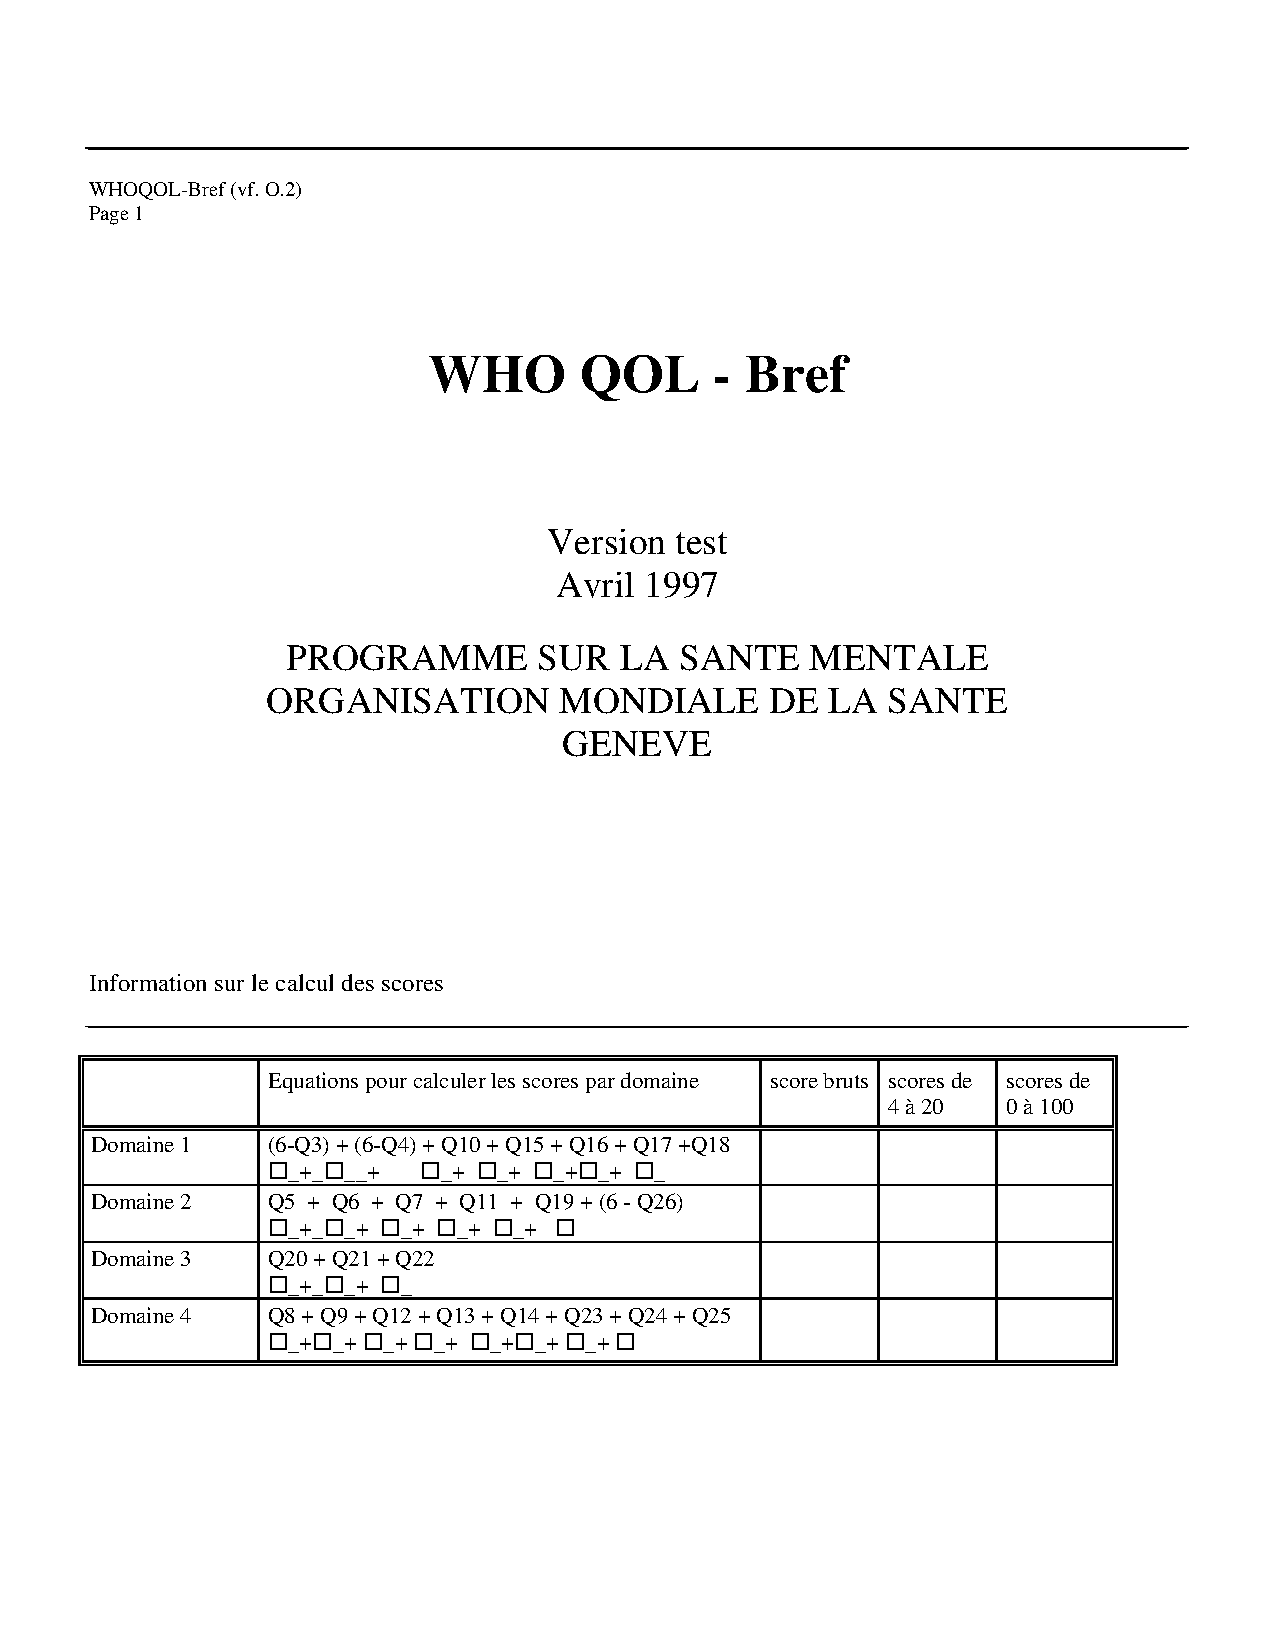
\includepdf[pages=-]{French_WHOQOL-BREF.pdf}
%
%\section{Questionnaire 2}
%
%
\includepdf[pages=-]{WHOQOLALLEMANDBREFupdated.pdf}

\chapter{Travail passif et actif de la méthode Tomatis}

\begin{description}
\item [{1\iere session}] de 25 à 30h d'écoute : le patient écoute
deux heures de musique par jour pendant 13 à 15 jours consécutifs;
un deuxième test à la fin de ce travail; ensuite, une pause pendant
4 à 6 semaines.
\item [{2\ieme session}] de 25 à 30h d'écoute : 3ieme Test, à nouveau
deux heures d'écoute pendant 13 jours à 15 jours; puis 4\ieme test,
suivi d'une pause d'une durée de 4 à 8 semaines.
\item [{3\ieme session}] : la même façon de procéder que les deux
autres. 
\end{description}

Le choix et le traitement des musiques peuvent être très différents
selon le patient et sa pathologie.
